\chapter{System Design}
\label{cha:system}
\vspace{0.4 cm} 

In this chapter, the methodology and the choices in the system design are presented. Starting by describing the components of the system with their functionalities (the blocks in the system architecture) and then explaining the working logic of the developed system. After this section, it will be clear which are the main parts of this system and how they cooperate to achieve the project goal.


\section{System architecture}
\label{sec:sysarc}
\vspace{0.2 cm} 

In a place of interest, there are people/users with their devices that are sending Wi-Fi packets, if they have the Wi-Fi device turned on. The purpose of our system is to exploit these packets to infer the number of people present. The system architecture of the developed system is shown in figure~\ref{fig:architecture}.
This is a distributed architecture, in fact, there are three main components on different platforms that cooperate over a communication network in order to achieve this goal.

\begin{figure}[h]
\centering 
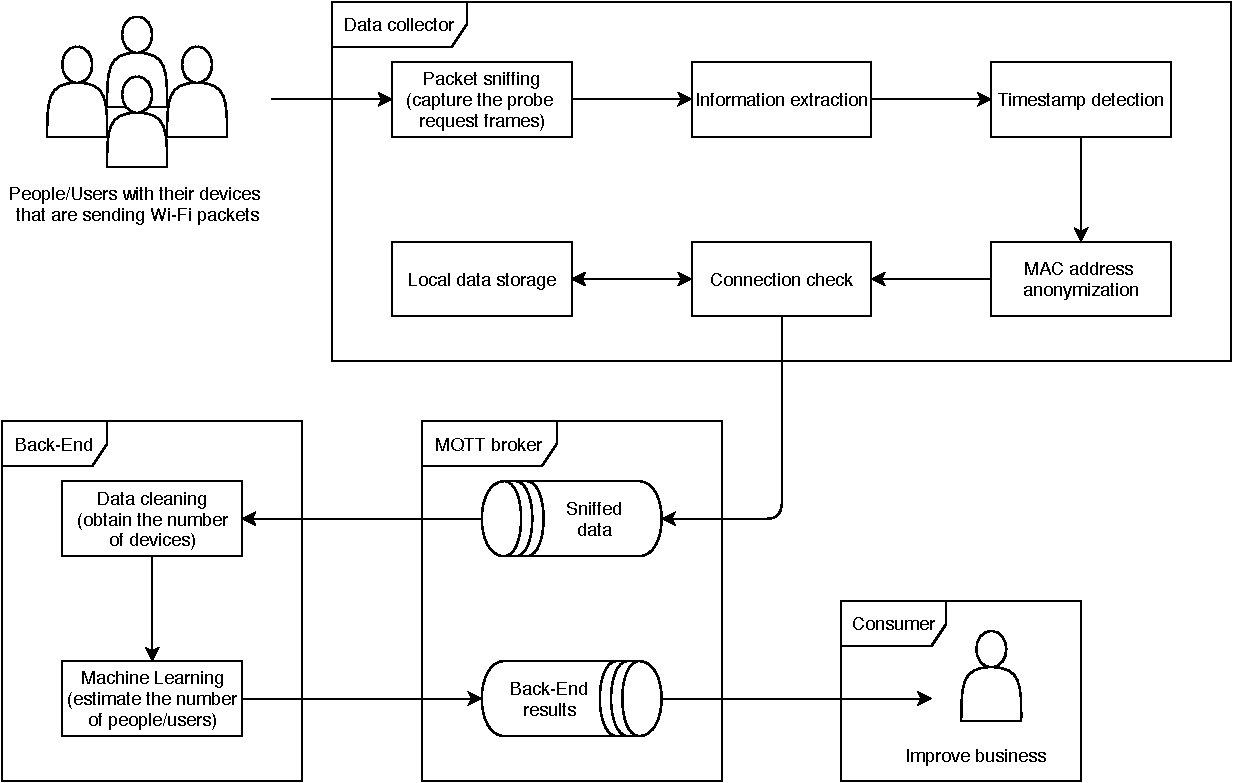
\includegraphics[width=0.9\textwidth]{images/architecture} 
\caption{Architecture of the proposed system.}
\label{fig:architecture}
\end{figure}

The first block of the system is a data collector (implemented on a Raspberry Pi 2B) which is located in the place of interest. It performs a preprocessing of the data (distributed work) with its functionalities: sniffing of Wi-Fi packets, capture the probe request frames; extract the useful information from these; detect the current timestamp; anonymize the MAC address using a hash function (no more privacy issues); check the internet connection; if there is no connection, save the data in the local storage; if there is a connection, publish the collected data to the dedicated queue (Collected data).

The system uses the MQTT protocol for data forwarding, an MQTT broker (situated TBD, it must have a static IP address to be accessible, implemented using Mosquitto MQTT broker) with 2 dedicated queues: one for the collected data (published by the data collector and received by the subscribed Back-End) and the other one for the Back-End results (published by the Back-End and received by the subscribed consumer).

The Back-End (situated TBD, implemented on a pc/server or running on Google Colaboratory) deals with collected data cleaning -- (to be decided based on the use case/case study: RSSI thresholding) remove random encounters (and randomized addresses are removed with this), make a blacklist to remove the ever-present devices or devices revealed too many times during the day and then get the number of devices present in the place of interest --, data analysis using Machine Learning -- fit the degree and the coefficients of the polynomial approximation using the trend and the seasonality of the number of devices detected to obtain the number of people present -- and publication of the results to the dedicated queue (Back-End results).

At the end of this processing, there is the consumer who receives the results of the Back-End, the number of people/users in the place of interest, and could use this information to improve his business.

This architecture is scalable, it could admit many sensors physically distributed in different environments for data collection, to provide a practical example some use cases are shown in figure~\ref{fig:excases}. It is important to locate them properly in the environments to cover all the areas of interest. All sensors publish data to the same MQTT broker and then all data is forwarded to the same Back-End. Cleaning and analysis will be performed according to the data source, each sensor will publish data in its own reserved queue and will be analyzed adequately to the characteristics of the use case for which it was used. (in the end, they are sent to the respective consumer through an appropriate queue)

\begin{figure}[h]
\centering 
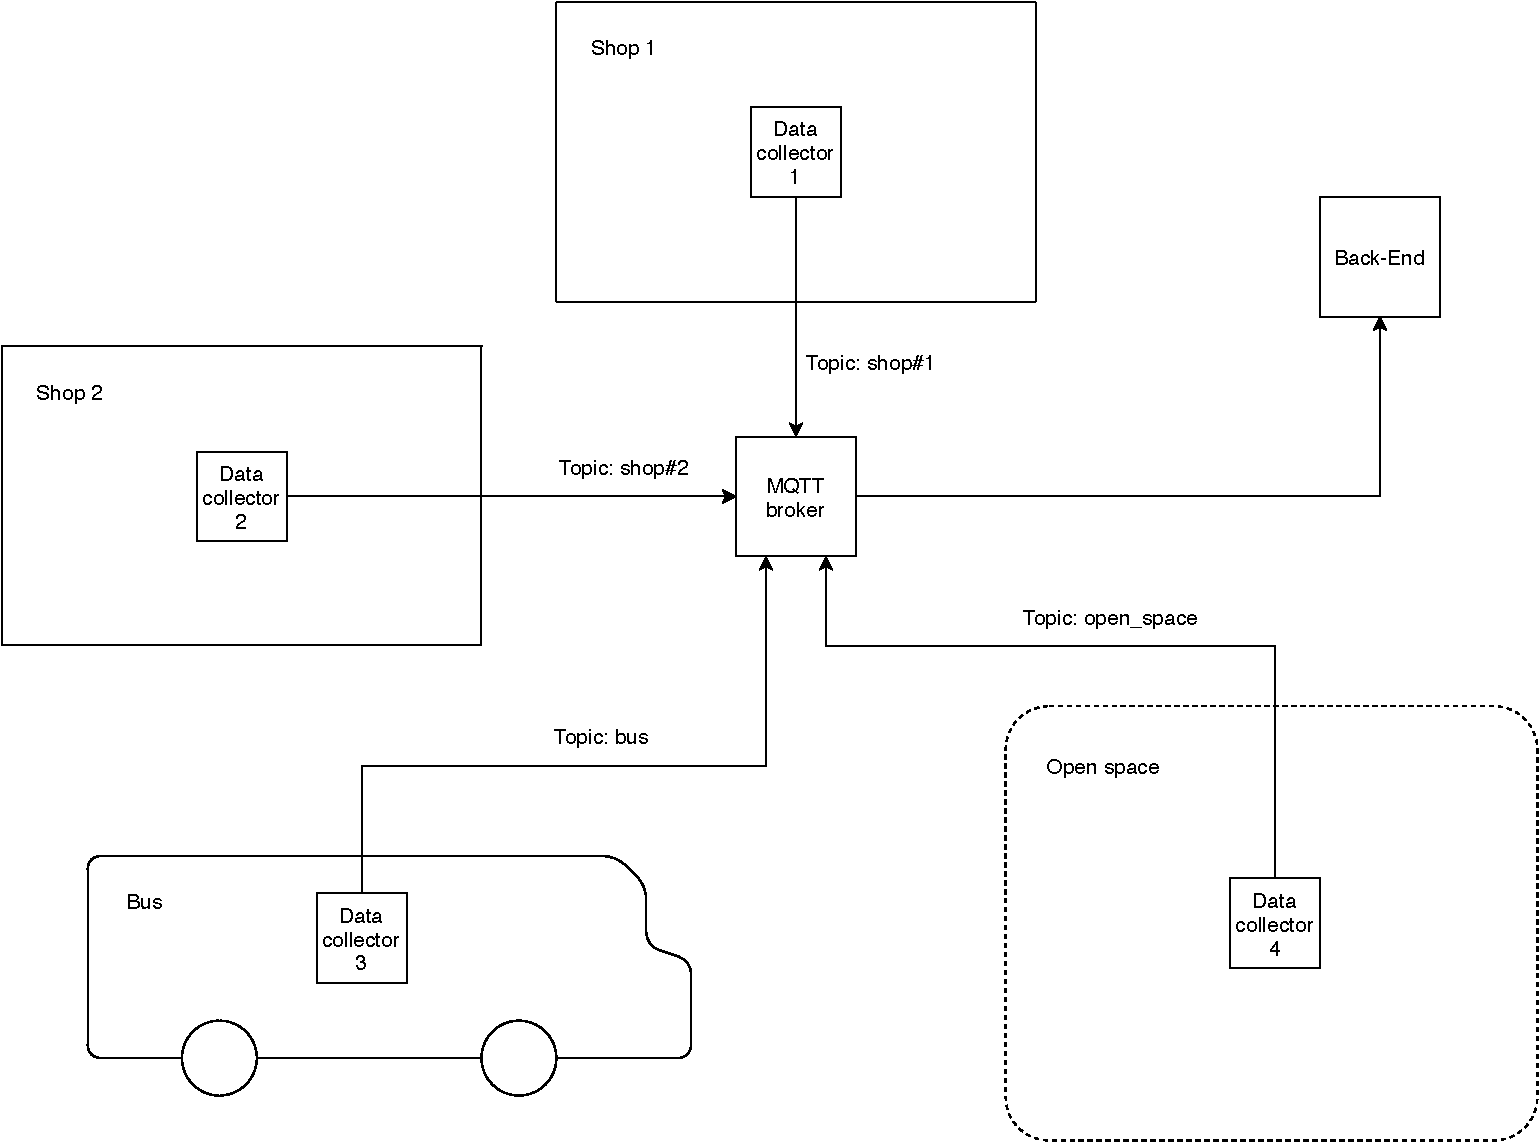
\includegraphics[width=0.9\textwidth]{images/excases} 
\caption{Presentation of a possible implementation with different use cases.}
\label{fig:excases}
\end{figure}


\section{Data collection}
\label{sec:collection}
\vspace{0.2 cm} 

The main block I worked on is the data collector. I developed the logic behind this block, with particular attention in the research of the connection and in the management of the data collected.

The flowchart representing the data collector logic is shown in figure~\ref{fig:flowcollect}. When the data collector is turned on, the system searches for the connected Wi-Fi dongle and puts it in monitor mode to perform the packet sniffing. Initially, a packet counter is set = 0 and the actual time is saved. When a packet is received, it checks if it is a probe request frame and if it is not, it is thrown away (using Scapy).
When a probe request frame is captured, the following information are extracted: RSSI, SSID (Service Set Identifier), MAC address, sequence counter. The timestamp when the packet was revealed is given by an RTC (Real Time Clock) board and together with the other information are saved temporarily in the RAM (Random Access Memory). The packet counter increases by one.


\begin{figure}[h!]
\centering 
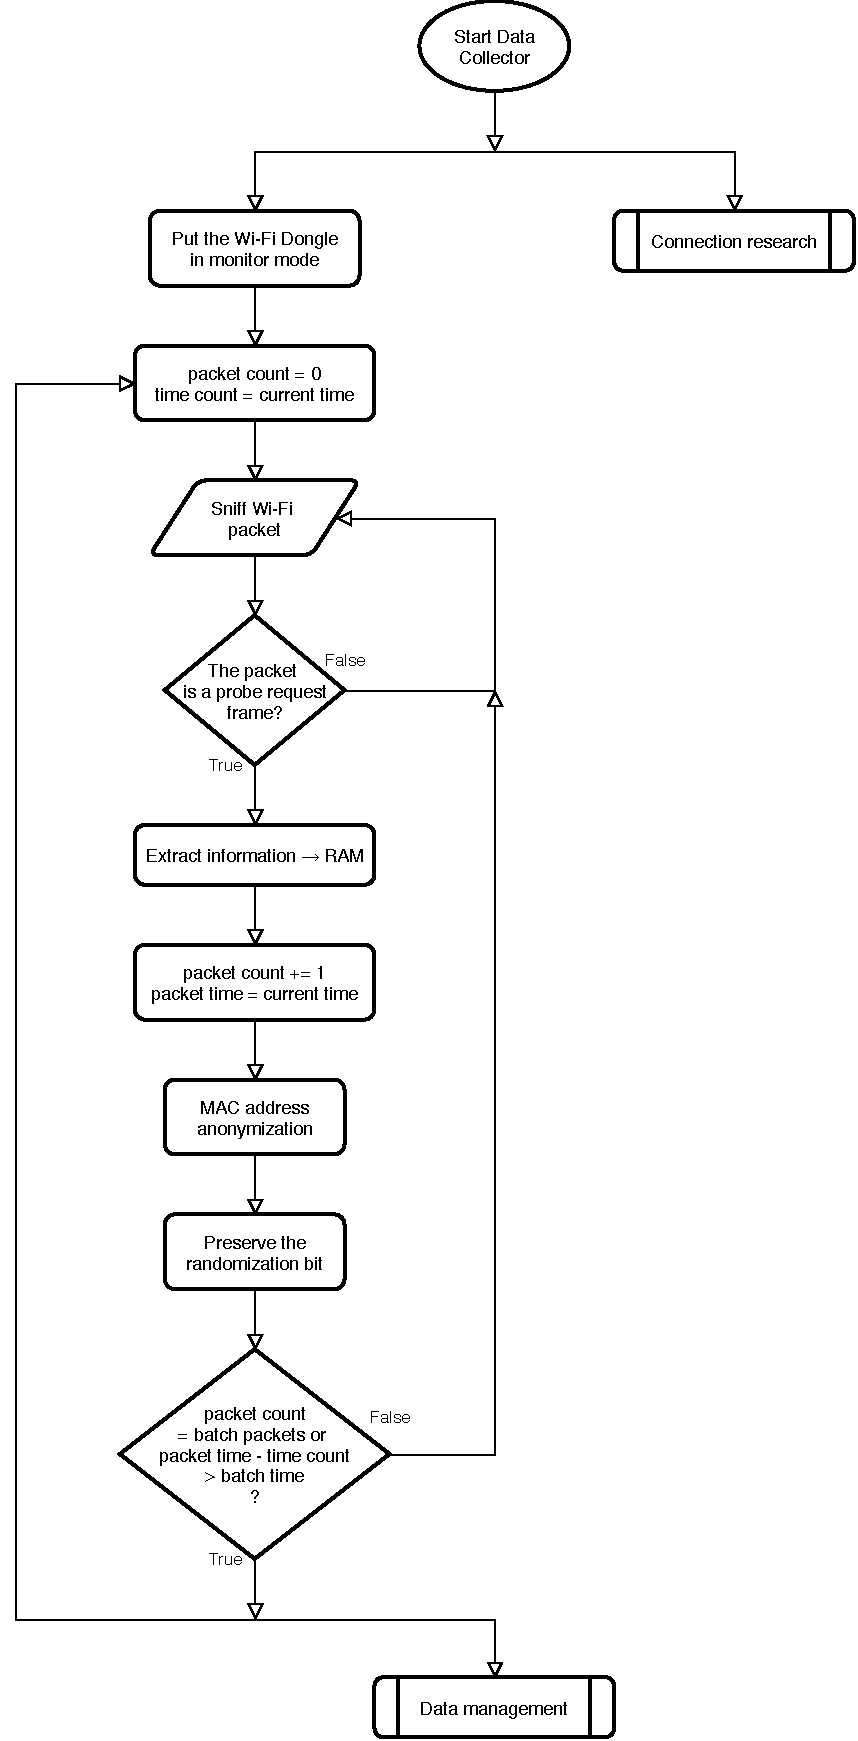
\includegraphics[width=0.62\textwidth]{images/flowcollect} 
\caption{Flowchart representing the data collector logic.}
\label{fig:flowcollect}
\end{figure}

% \begin{wrapfloat}{figure}{I}{0pt} 
% 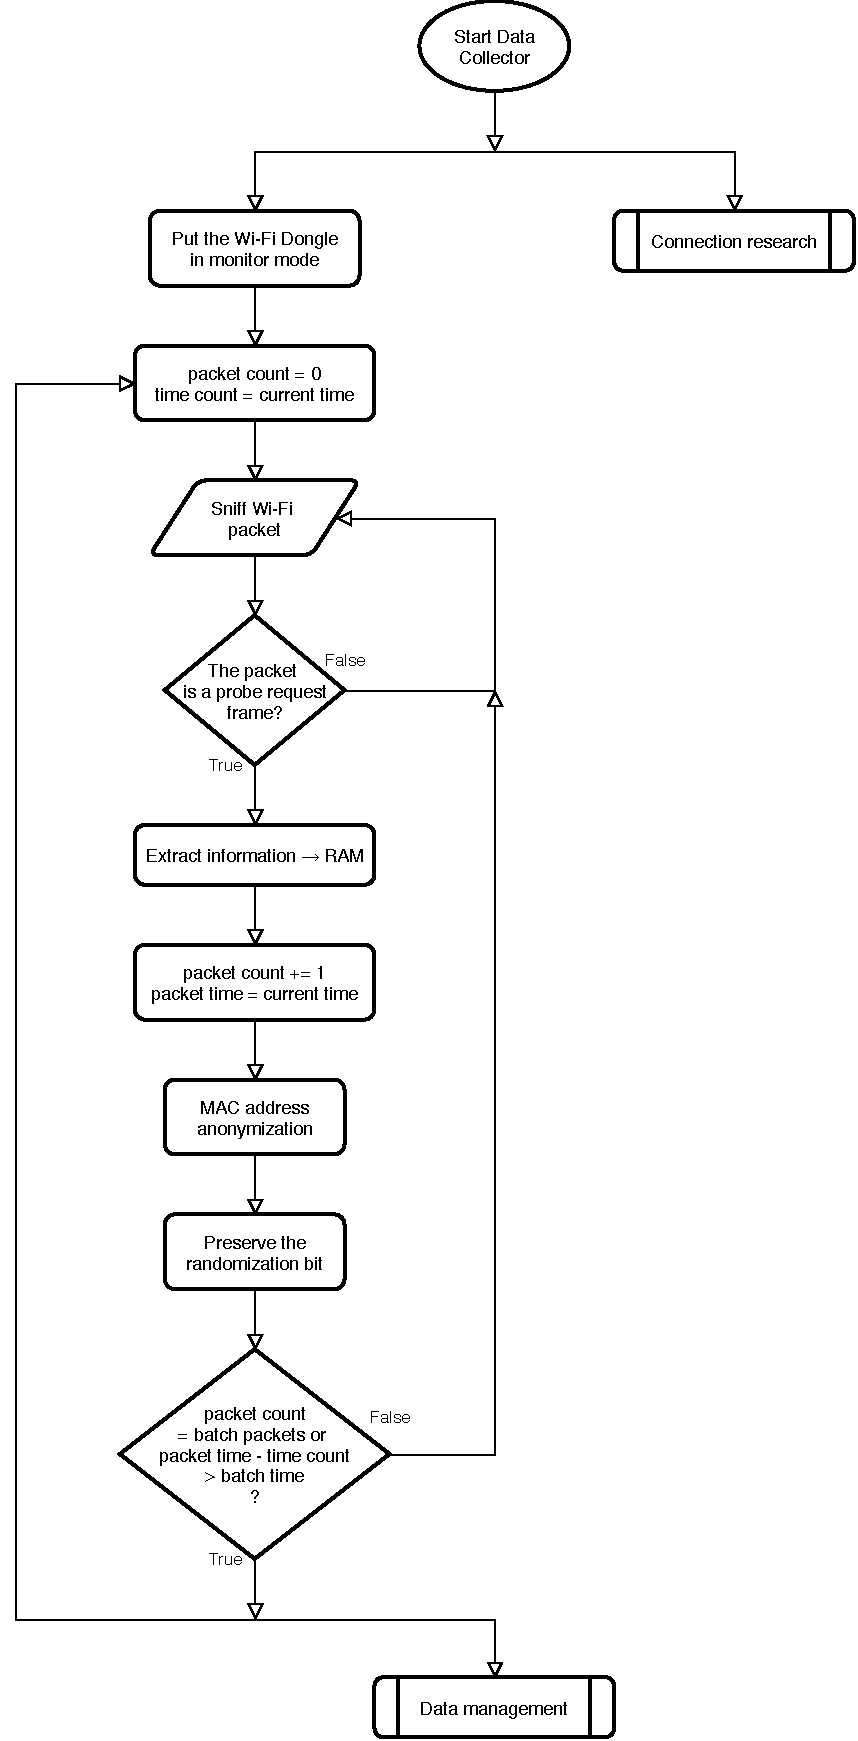
\includegraphics[width=0.5\textwidth]{images/flowcollect}
% \caption{Flowchart representing the data collector logic.}
% \label{fig:flowcollect}
% \end{wrapfloat}

Among the information that can be extracted from the MAC address before performing the anonymization there are the OUI (Organizationally Unique Identifier), from which the manufacturer of the device can be identified, and the local bit, the 7\textsuperscript{th} bit of the MAC address, from which it can be seen whether the MAC address is randomized or not.

After extracting the information, there is the anonymization of the MAC address to preserve the privacy of the users and comply with the GDPR. This is made only for the MAC addresses that are not randomized, i.e. the real MAC addresses of the devices present. Anonymization is performed at this point in the architecture because then there are no more privacy problems, this work does not have to be done from the Back-End and for reasons of data security in case of a data breach during transmission.
This process consists of hashing the MAC address using BLAKE2s, an implementation of the BLAKE2 cryptographic hash function based on BLAKE \footnote{ website: https://blake2.net/ } (BLAKE3 is faster but still under development). BLAKE2 is faster than MD5, SHA-1, SHA-2 and SHA-3, and provides security superior to SHA-2 and similar to that of SHA-3. BLAKE2 supports keying and salting, and can output digests from 1 up to 32 bytes for BLAKE2s. This hash function is the ideal for changing hash results every 24 hours or predefined time, simply modifying the key or adding a different value of salt. This is made for privacy reasons and to avoid tracing the MAC address although it is not the real one but always the same after hashing.
If the anonymization changes the state of the local bit, the previous state is forced/imposed to preserve this information on randomization, which can be used in the cleaning phase.

Once the pre-processing of the data is completed, we decided to process the collected data in batches and therefore there are to check 2 batch criteria, based on a maximum number of packets and a maximum time since the last batch transmission. These parameters have to be set according to the use case/case study, once one of these is reached it is possible to decide what to do with this data by running the data management flowchart (shown in figure~\ref{fig:flowdata}).

\begin{figure}[h]
\centering 
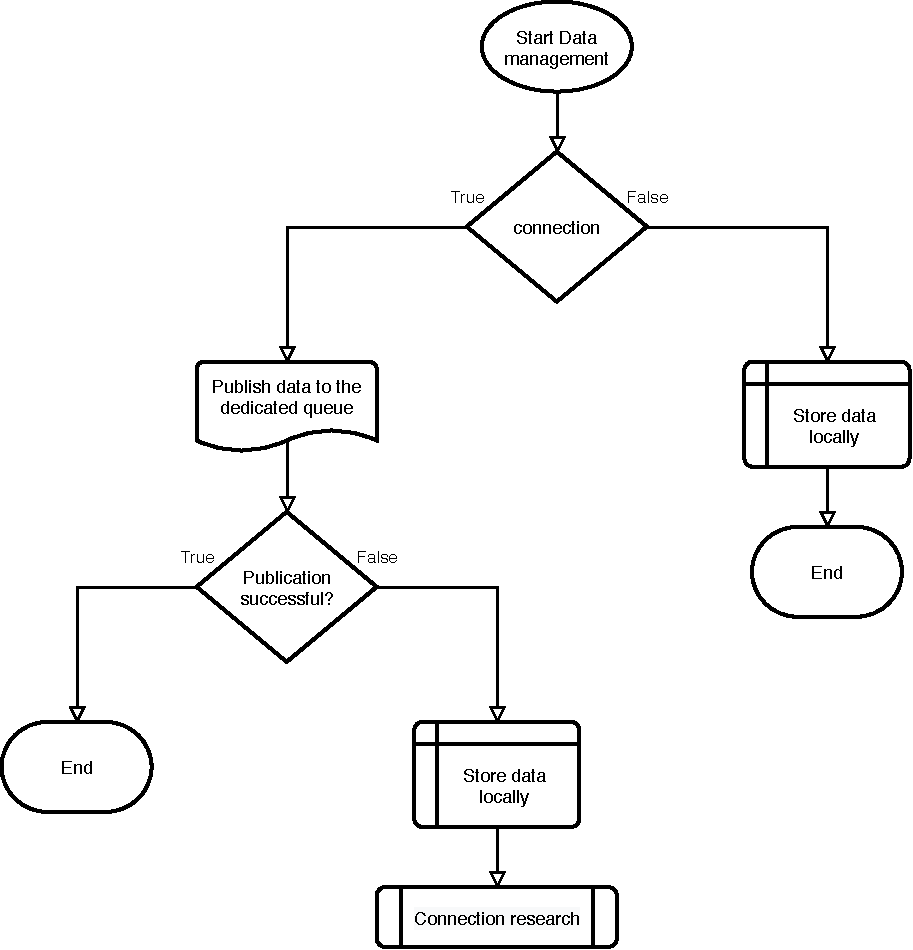
\includegraphics[width=0.6\textwidth]{images/flowdata} 
\caption{Flowchart representing the data management logic.}
\label{fig:flowdata}
\end{figure}

Higher values of the parameters allow us to avoid a continuous transmission of data and to fill the queue on the broker or in the lack of a connection, to open the file to save the data every time a packet is detected. On the other hand, choosing smaller values of the parameters reduces estimation delay, making the system more responsive. In our experiments, we used intermediate values with a maximum number of packets of 50 and a maximum time since the last batch transmission of 60 seconds, which is a good trade-off between congestion and transmission delay.

When the batch is ready, the algorithm for managing what to do with the data starts. If there is no connection, the collected data is stored locally (using json.dump()) to be sent later when a connection is found. After that, the data is deleted from the RAM.
Instead, if there is a connection with the MQTT broker, the collected data is published to the dedicated queue (Collected data, converted in a string using json.dumps() to be published). If the publication is successful, the data is deleted from the RAM. Otherwise, it is stored locally (using json.dump()), subsequently deleted from the RAM and finally the system searches again for a connection.

\begin{figure}[h]
\begin{minipage}[b]{8.5cm}
\centering
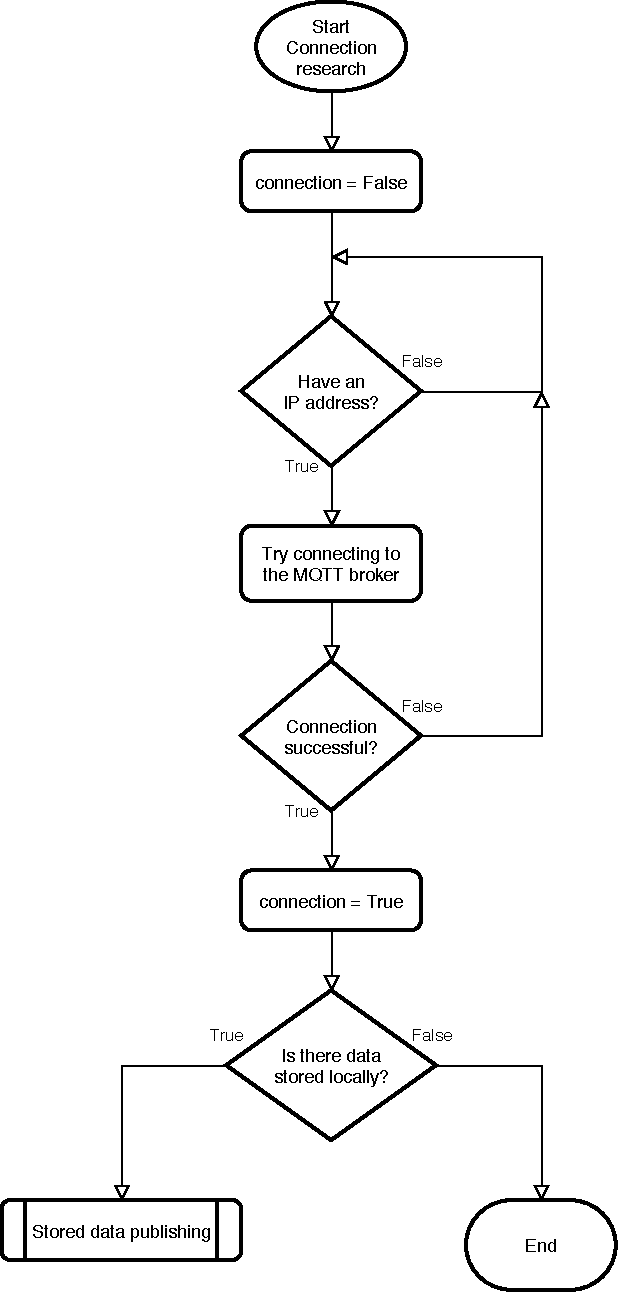
\includegraphics[width=0.97\textwidth]{images/flowconnection}
\caption{Flowchart representing the connection research logic.}
\label{fig:flowconnection}
\end{minipage}
\ \hspace{2mm} \hspace{3mm} \
\begin{minipage}[b]{8.5cm}
\centering
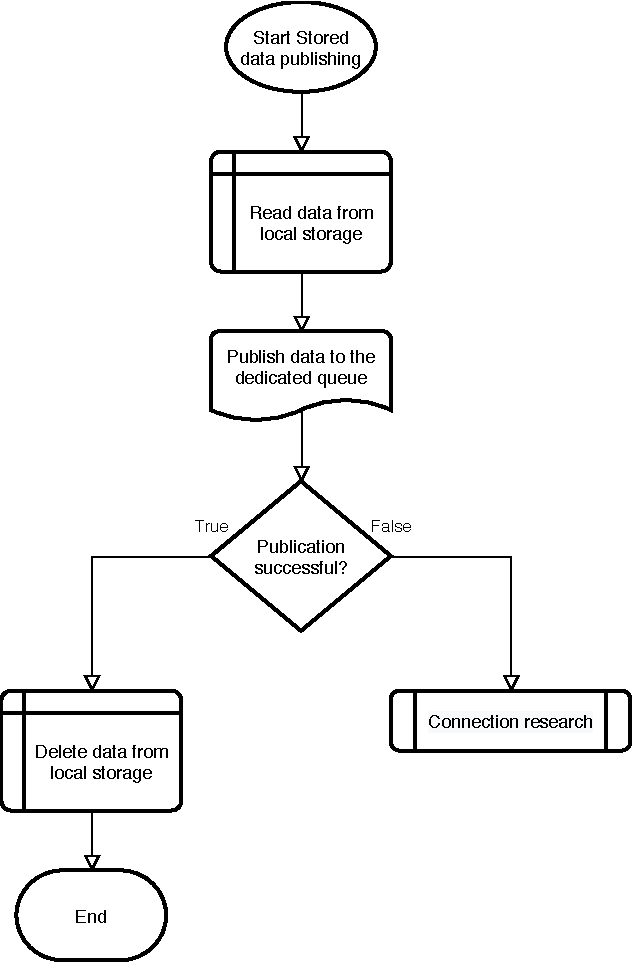
\includegraphics[width=0.97\textwidth]{images/flowstorage}
\caption{Flowchart representing the stored data publishing logic.}
\label{fig:flowstorage}
\end{minipage}
\end{figure}

% \begin{figure}[h]
% \centering 
% 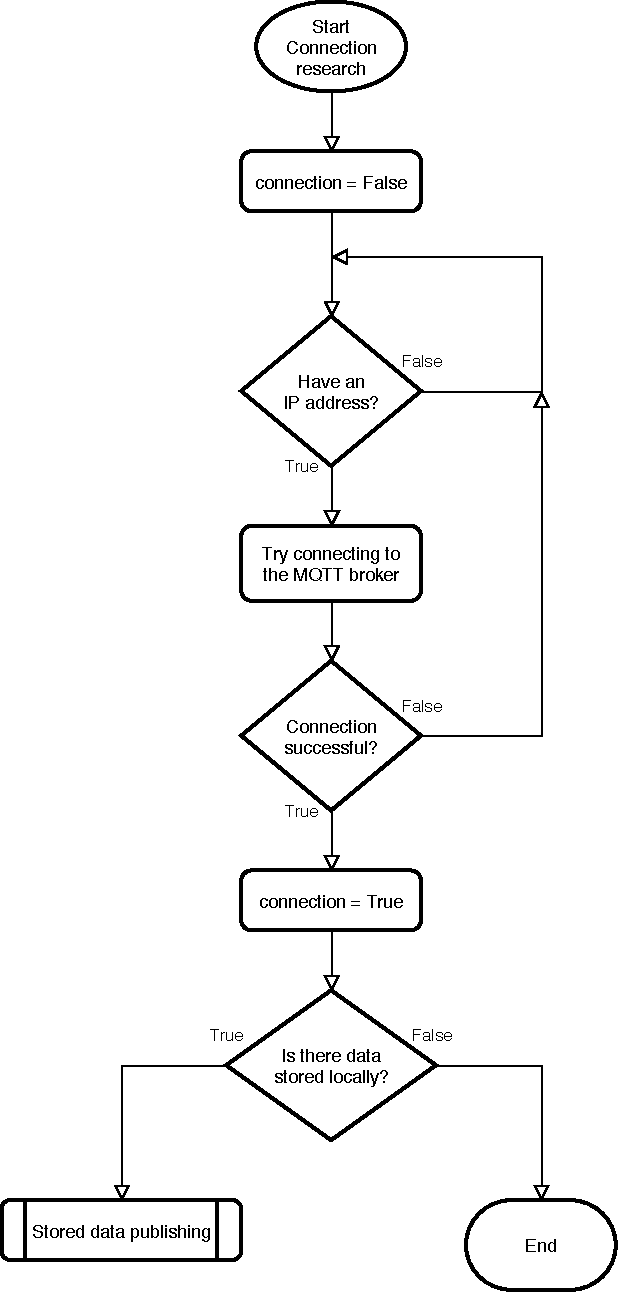
\includegraphics[width=0.5\textwidth]{images/flowconnection} 
% \caption{Flowchart representing the connection research logic.}
% \label{fig:flowconnection}
% \end{figure}

When the data collector is turned on, the system searches also for a connection with the MQTT broker. Figure~\ref{fig:flowconnection} shows the flowchart explaining the logic behind this. Initially, the connection is set = False and the system checks whether the data collector has a peripheral with an IP address for Internet access.
When it has an IP address, a Paho MQTT Client with its credentials tries connecting to the MQTT broker. When the broker is reachable and accepts the client connection, the connection is set = True and if there is data stored locally, it can be published by running the flowchart for the publication of the stored data (shown in figure~\ref{fig:flowstorage}).

% \begin{figure}[h]
% \centering 
% 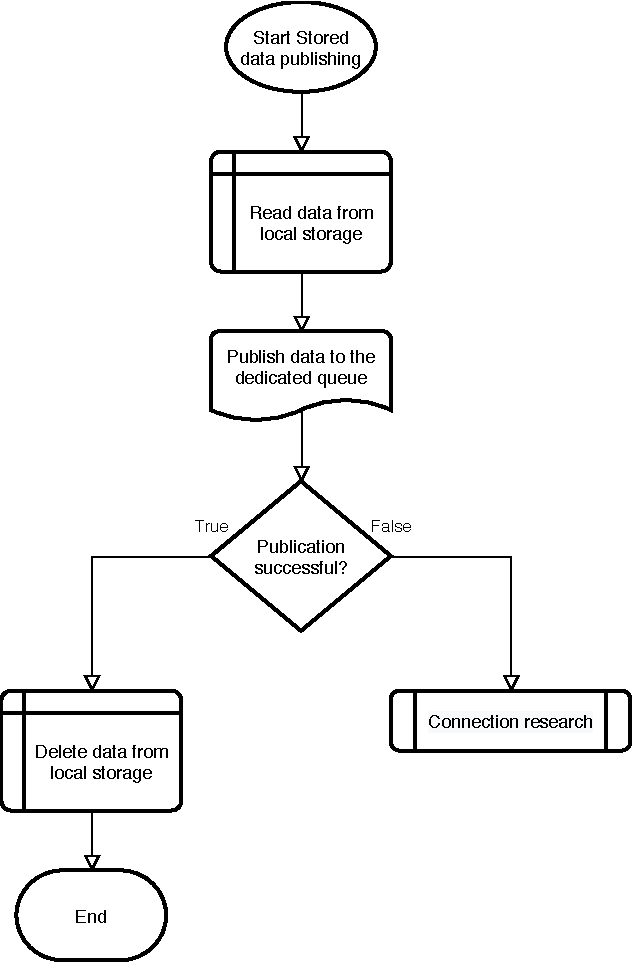
\includegraphics[width=0.5\textwidth]{images/flowstorage} 
% \caption{Flowchart representing the stored data publishing logic.}
% \label{fig:flowstorage}
% \end{figure}

The data is read from the local storage (using json.loads()) and is published to the dedicated queue (Collected data, converted in a string using json.dumps() to be published).
If the publication is successful, the data is deleted from the local storage. Otherwise, it remains stored locally and the system searches again for a connection.


\section{Data forwarding}
\label{sec:forwarding}
\vspace{0.2 cm} 

MQTT \footnote{ website: http://mqtt.org/ } stands for Message Queuing Telemetry Transport. It is a publish/subscribe, extremely simple and lightweight messaging protocol. It is designed to be bandwidth-efficient and to use little battery power. It is efficient in distributing information to one or many receivers. Information is organized in topics. Topics are treated as a hierarchy, using a slash (/) as a separator. These principles make it the ideal protocol for the emerging world of machine-to-machine/Internet of Things and for mobile applications where bandwidth and battery power are limited. It is useful for connections with remote locations, as in our case to send a huge amount of data to the Back-End. Moreover, it can easily scale from a single device to thousands

The MQTT protocol defines two types of network entities: a message broker and clients. An MQTT broker is a software (in our case we used Mosquitto) running on a computer that receives all messages from the clients and then routes them to the appropriate destination clients. An MQTT client is any device that runs an MQTT library (in our case we used paho-mqtt for Python) and connects to an MQTT broker over a network.
For security reasons, the MQTT broker can be configured to require clients to use a username and password when connecting. If they match allowed credentials, clients can publish/subscribe to the topics. Otherwise, the connection is refused.
When a publisher has new data to distribute, it publishes this data to the broker. Any client that wants a copy of that message will subscribe to that topic. The broker then distributes the data to any clients that have subscribed to that topic. Multiple clients can receive the message from a single broker. Similarly, multiple publishers can publish topics to a single subscriber.

The protocol uses a publish/subscribe architecture in contrast to HTTP with its request/response paradigm. The main difference to HTTP is that a client does not have to pull the information it needs, but the broker pushes the information to the subscribed client, in case something new has been published. The broker also keeps track of all session information as clients connect and disconnect. If this connection is interrupted by any circumstances, the MQTT broker can buffer all messages and send them to the client when it is back online, setting the clean session bit = False. If clean session bit is true, then all subscriptions will be removed for the client when it disconnects.

Each subscription/publication to the broker can specify a quality of service measure. These are classified in increasing order of overheads:
\begin{itemize}
  \item 0: At most once - the message is sent only once and the publisher and broker take no additional steps to acknowledge delivery to the subscribers (fire and forget, with no confirmation).
  \item 1: At least once - the message is re-tried by the sender (publisher or broker) multiple times until acknowledgment is received (by the broker or the subscribers) (acknowledged delivery).
  \item 2: Exactly once - the sender (publisher or broker) and receiver (broker or the subscribers) engage in a two-level handshake to ensure only one copy of the message is received (assured delivery).
\end{itemize}

For these illustrated features, the MQTT protocol is used in the system for data forwarding. A broker (situated TBD, it must have a static IP address to be accessible, implemented using Mosquitto MQTT broker) with two dedicated queues is used, one for the collected data (published by the data collector and received by the subscribed Back-End) and the other one for the Back-End results (published by the Back-End and received by the subscribed consumer).
The broker is set up to allow only connections from the data collector, the Back-End and the consumer. They have their own credentials for authentication.

Client(client\_id=``name'', clean\_session=False), connect(``broker\_address'', port=1883)

username\_pw\_set(``username'', password=``password'')

publish(``topic'', payload=json.dumps(data), qos=2)

subscribe(``topic'', qos=2)

The clean\_session is set = False. If this connection is interrupted by any circumstances, the MQTT broker can buffer all messages and send them to the client when it is back online.
The QoS is set = 2 both in publish and subscribe. To ensure exactly one copy of the data, no loss, no duplicates to clean. Data is converted in string using json.dumps() to be published and forwarded.


\section{Data cleaning and analysis}
\label{sec:analysis}
\vspace{0.2 cm} 

The two main Back-End functionalities are data cleaning and data analysis.(situated TBD, implemented on a pc or running on Google Colaboratory)

The flowchart representing the data Back-End logic is shown in figure~\ref{fig:flowcleaner}. Initially, the Back-End subscribes to the collected data queue to receive the data when published by the data collector. Input data is managed by adding corollary information for future analysis and is stored locally.

\begin{figure}[h]
\centering 
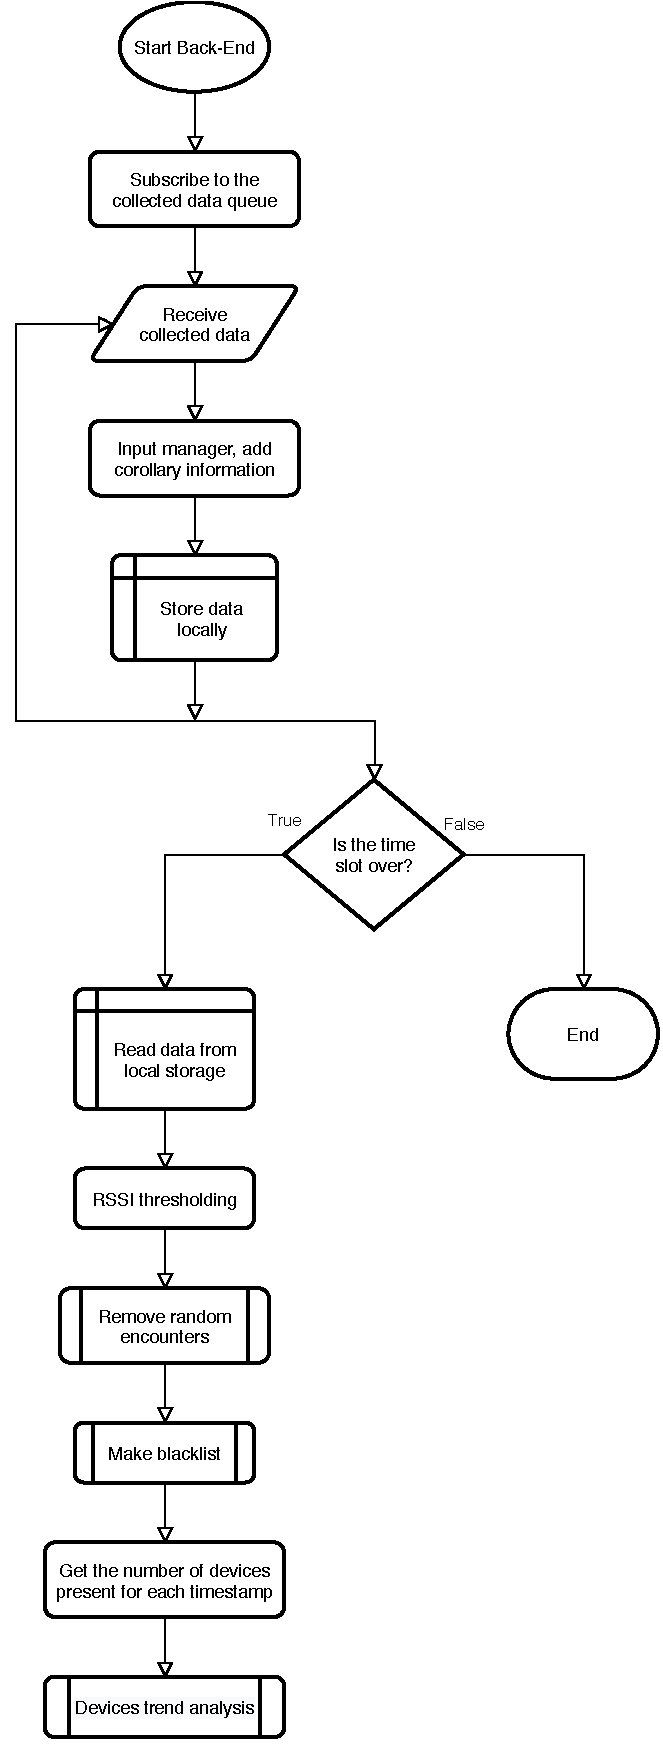
\includegraphics[width=0.5\textwidth]{images/flowcleaner} 
\caption{Flowchart representing the Back-End and the cleaning logic.}
\label{fig:flowcleaner}
\end{figure}

When a time slot is over, the data of the current time slot is read from the local storage. An RSSI-based threshold is applied to delete data from devices too far from the data collector (to be decided based on the use case/case study, the position of the data collector has to be taken into consideration, as well the environment in which they are located, for cleaning and analysis). Random encounters are removed, as shown in the flowchart in figure~\ref{fig:flowrandom}. Unique devices are extracted with their occurrence timestamps. If there are devices that appear only once or for a short time, they are removed. These parameters have to be adapted at the use case/case study (and randomized addresses are removed with this).

% \begin{figure}[h]
% \centering 
% 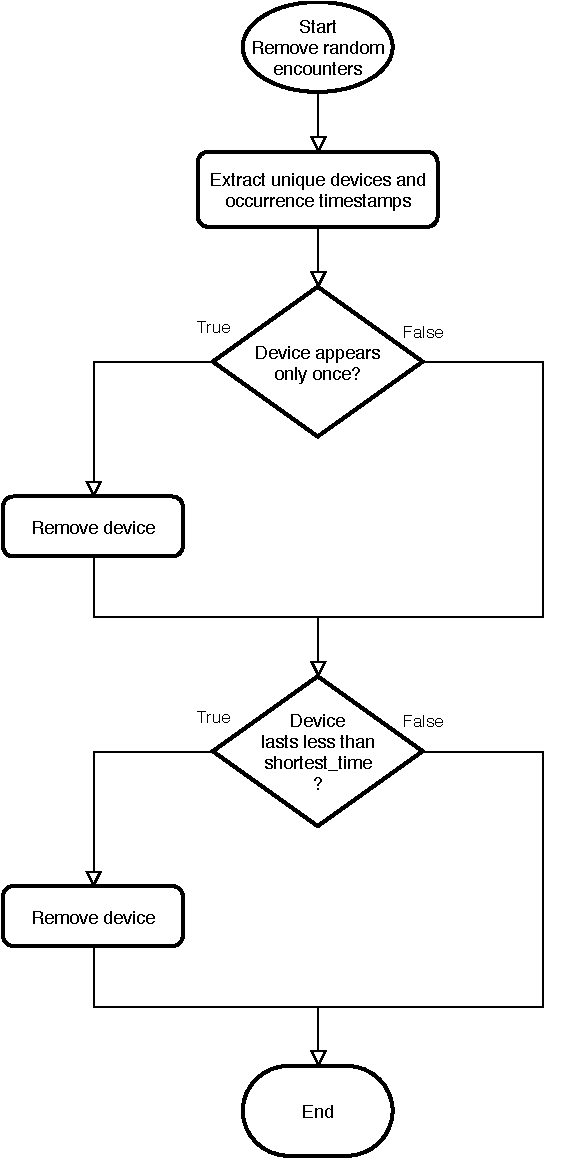
\includegraphics[width=0.5\textwidth]{images/flowrandom} 
% \caption{Flowchart representing the logic of removing casual encounters.}
% \label{fig:flowrandom}
% \end{figure}

Then a blacklist is made to remove the ever-present devices or devices revealed too many times during the day, as shown in the flowchart in figure~\ref{fig:flowblacklist}. A list of occurrences is created with a maximum interrupt time of delta\_t. If there are devices that appears many times or for a long time, they are blacklisted. These parameters have to be adapted at the use case/case study.
At this point, it is possible to get the number of devices present in the place of interest for each timestamp based on the occurrences of the devices not in the blacklist.

% \begin{figure}[h]
% \centering 
% 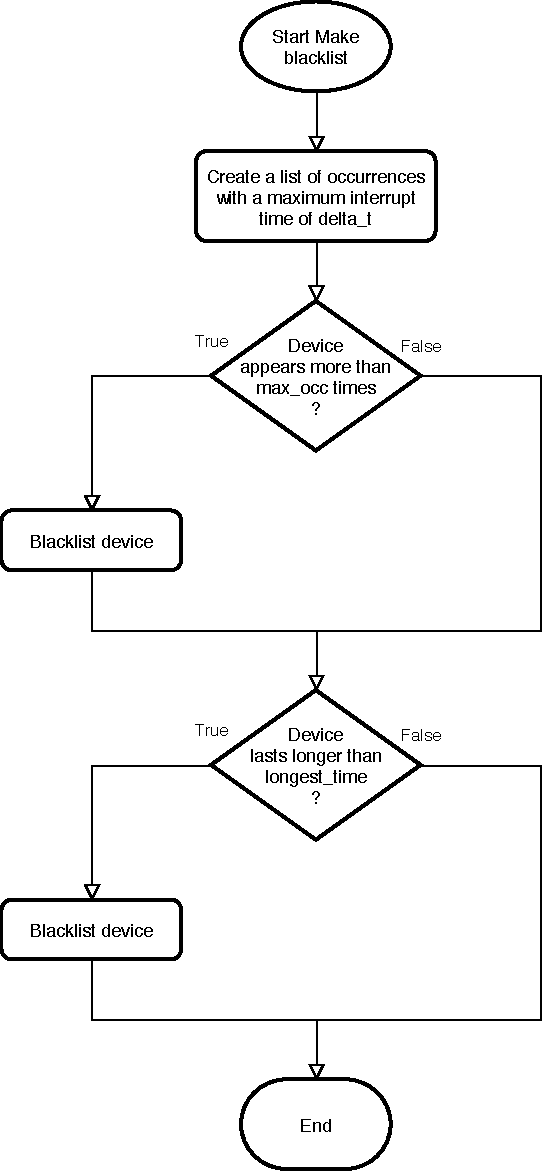
\includegraphics[width=0.5\textwidth]{images/flowblacklist} 
% \caption{Flowchart representing the logic of making the blacklist.}
% \label{fig:flowblacklist}
% \end{figure}

\begin{figure}
\begin{minipage}[b]{8.5cm}
\centering
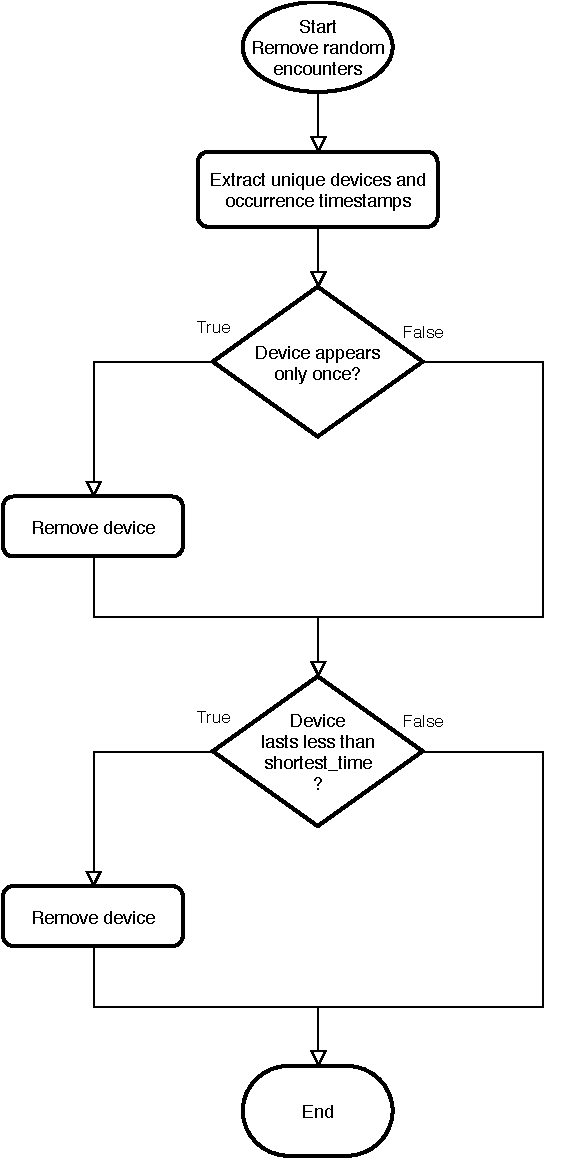
\includegraphics[width=0.9\textwidth]{images/flowrandom}
\caption{Flowchart representing the logic of removing casual encounters.}
\label{fig:flowrandom}
\end{minipage}
\ \hspace{2mm} \hspace{3mm} \
\begin{minipage}[b]{8.5cm}
\centering
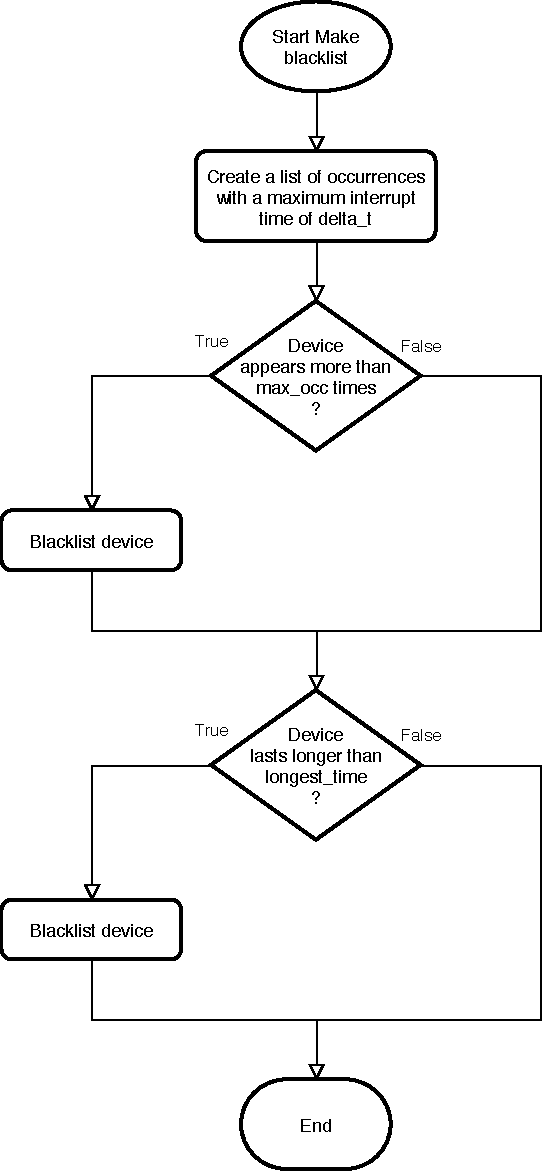
\includegraphics[width=0.9\textwidth]{images/flowblacklist}
\caption{Flowchart representing the logic of making the blacklist.}
\label{fig:flowblacklist}
\end{minipage}
\end{figure}

Finally, data analysis is performed, as shown in the flowchart in figure~\ref{fig:flowML}. Trend (raising/lowering) and seasonality (repetition of the components) of the number of devices are extracted using a decomposition of the corresponding temporal series. Once these two variables are known, it is possible to apply to them the correct polynomial approximation relating to the current time slot to get the forecast of the people present in the place of interest. The best degree and coefficients of the polynomial approximation are calculated during the training phase/preparation of the model for each time slot of each day of the week, using manually-collected ground truth. Figure~\ref{fig:flowtrainML} shows the flowchart of the logic used in that phase.

% \begin{figure}[h]
% \centering 
% 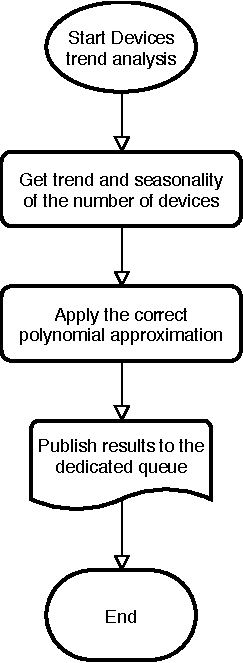
\includegraphics[width=0.3\textwidth]{images/flowML} 
% \caption{Flowchart representing the data analysis logic.}
% \label{fig:flowML}
% \end{figure}

% \begin{figure}[h]
% \centering 
% 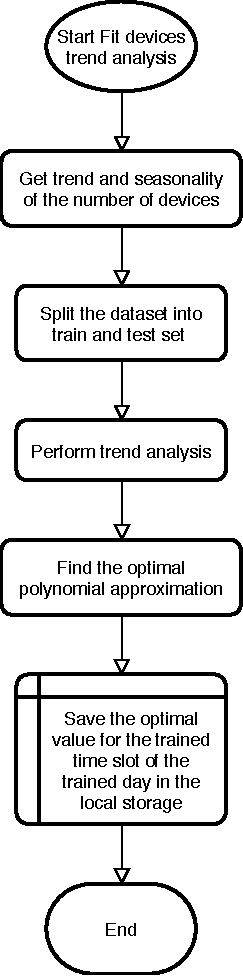
\includegraphics[width=0.3\textwidth]{images/flowtrainML} 
% \caption{Flowchart representing the ML training logic.}
% \label{fig:flowtrainML}
% \end{figure}

\begin{figure}
\begin{minipage}[b]{8.5cm}
\centering
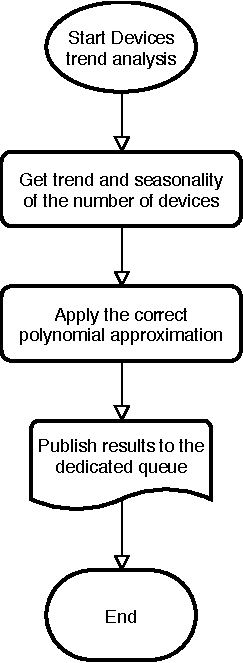
\includegraphics[width=0.6\textwidth]{images/flowML}
\caption{Flowchart representing the data analysis logic.}
\label{fig:flowML}
\end{minipage}
\ \hspace{2mm} \hspace{3mm} \
\begin{minipage}[b]{8.5cm}
\centering
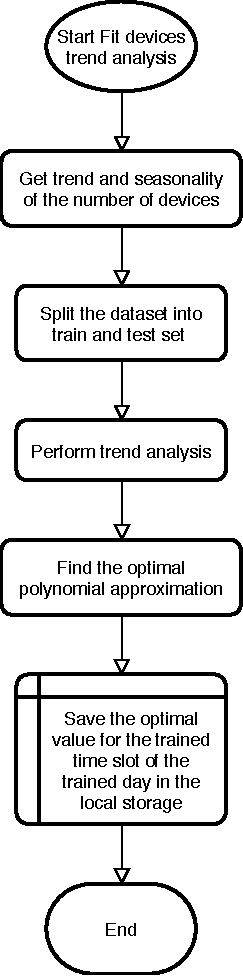
\includegraphics[width=0.6\textwidth]{images/flowtrainML}
\caption{Flowchart representing the ML training logic.}
\label{fig:flowtrainML}
\end{minipage}
\end{figure}

I did not develop the part of machine learning, but I integrated an existing one into this project to get the final results, i.e. the number of people/users in the place of interest for each timestamp. Then the results, when available, are published to the dedicated queue (Back-End results) to be received by the subscribed consumer who could use this information to improve his business.
